\begin{center}
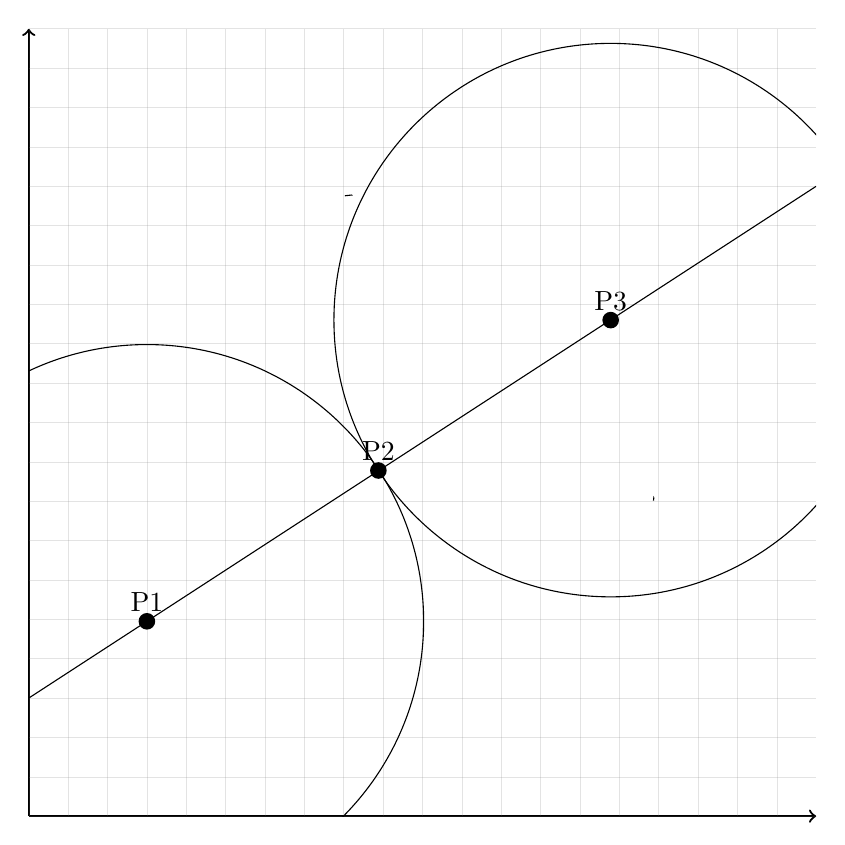
\begin{tikzpicture}
	[scale = 1,
	axis/.style={->, black, thick}]
	
	% Draw main axes
	\draw[axis] (0, 0) -- (10, 0);
	\draw[axis] (0, 0) -- (0, 10);
	
	\clip (0,0) rectangle (10, 10);
	
	% Draw grid
	\foreach \x in {0, 0.5, ..., 10.1}
		\foreach \y in {0, 0.5, ..., 10.1}
		{
			\draw[very thin, gray, opacity=0.01] (\x, 0) -- (\x, 10);
			\draw[very thin, gray, opacity=0.01] (0, \y) -- (10, \y);
		}
		
	% Draw path
	\draw[] (0, 1.5) -- (10, 8);
		
	% Draw first point
	\coordinate (P1) at (1.5, 2.475);
	\fill (P1) circle[radius=3pt] node[anchor=south]{P1};
	\draw (P1) circle[radius=100pt];

	% Draw second point
	\begin{scope}
		\coordinate (P2) at (4.44, 4.39);
		\fill (P2) circle[radius=3pt] node[anchor=south]{P2};
		\path[clip] (P2) -- (4.0, 8.0) -- (8.0, 4.0);
		\draw (P2) circle[radius=100pt];
	\end{scope}
	
	% Draw third point
	\coordinate (P3) at (7.39, 6.3);
	\fill (P3) circle[radius=3pt] node[anchor=south]{P3};
	\draw (P3) circle[radius=100pt];
	
	
	
\end{tikzpicture}
\end{center}